\section[Voronoi and Delaunay]{Voronoi Regions, Dirichlet Tessellations and Delaunay Triangulations}
\subsection{Motivation}
Given an arbitrary set of points in the 2D plane, a \textit{Voronoi Diagram} or \textit{Dirichlet Tessellation} divides the plane into tiles; each point is associated with the region of the plane closest to it.\\~\\
\begin{figure}[H]
    \centering
    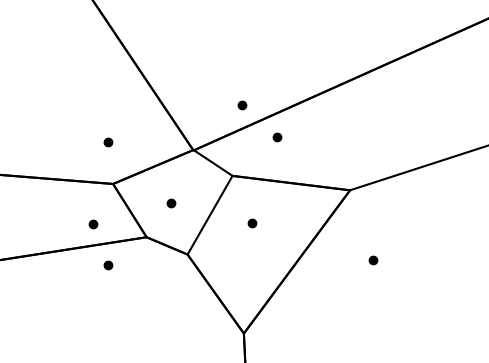
\includegraphics[width=0.7\textwidth]{voronoi.png}
    \caption{Points and their Voronoi regions}
    \label{fig:my_label}
\end{figure}
Voronoi diagrams are of monumental importance in many different branches of science and were rediscovered numerous times. Geographers speak of Thiessen polygons, which are used as models for crystal growth, while Metallurgists speak of Wigner-Seitz zones for analyzing equilibrium properties of alloys. As we see later, its dual graph, the \textit{Delaunay Triangulation}, also has various applications in other fields, for example as an automatic mesh generator used in finite element methods. Voronoi Diagrams are especially useful for many problems in the field of computational geometry.
\newpage
\cite{Aurenhammer1991} summarizes the importance as follows:
\begin{quote}
    Accordingly, Voronoi diagrams are useful in three respects: As a structure per se that makes explicit natural processes, as an auxiliary structure for investigating and calculating related mathematical objects, and as a data structure for algorithmic problems that are inherently geometric.
\end{quote}
For a more exhaustive list of applications, see \cite{Aurenhammer1991}.
\subsection{Definitions and Theorems}
We use the formal definitions provided by \cite{Green1978}.
\begin{definition}[Voronoi tile]
Let $\mathcal{P}_N := \{P_1, P_2, \dots, P_N\}$ be finitely many points in the plane such that $P_i \neq P_j, i\neq j$. The \textbf{Voronoi tile} of $P_i$ is the set $T_i$ defined by
\[
T_i = \{
  x : d(x, P_i) < d(x, P_j), \forall j \neq i
\}
\]
where $d$ is the euclidean distance.
\end{definition}
Note that tiles are infinite if and only if they are not entirely surrounded by other tiles. Further note that all tiles are trivially convex.\\
Not every point is part of a tile. Let $P_n$ and $P_m$ be 2 points and $T_n$, $T_m$ be their neighbouring tiles. If $x$ is a point such that $d(x, P_n) = d(x, P_m)$ then $x$ lies in neither $T_n$ nor $T_m$. This is why tiles are open, all points neighbouring 2 or more tile centers form the \textbf{boundary segments} of that tile.
\begin{definition}[Voronoi Diagram, Dirichlet Tessellations]
A \textbf{Voronoi Diagram}, also called a \textbf{Dirichlet Tessellation}, is the set of all tiles and boundaries subdividing a given space.
\end{definition}
Although intuitively understandable, let us formally define what a neighbour is:
\begin{definition}[Neighbour]
Two Voronoi Tiles are \textbf{neighbours} if and only if they share one boundary segment.
\end{definition}
Through Voronoi diagrams, we can easily get another important geometric structure.
\begin{definition}[Triangulation]
A \textbf{triangulation} is a subdivision of an object into simplicies. Note that in 2D, this is a subdivision into triangles.
\end{definition}
\begin{definition}[Delaunay Triangulation]
Let $\mathcal{P}_N$ be finitely many points in the plane, no two of which coincide. Further let $T_1, \dots, T_n$ be the Voronoi tiles of those points. The \textbf{Delaunay Triangulation} is a triangulation of these points with the following property:
\[
\forall i,j \in \{1,\dots,n\}, i \neq j: (P_i, P_j) \text{ are connected } \Leftrightarrow (T_i, T_j) \text{ are neighbours }
\]
This makes the Delaunay Triangulation the \textbf{dual graph} of the Voronoi Diagram (See \cite{FORTUNE1995}, Theorem 2.1.3)
\end{definition}
\begin{figure}[H]
    \centering
    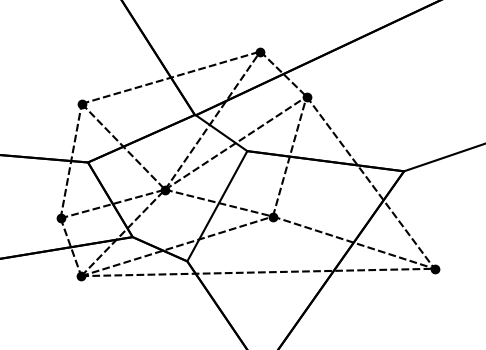
\includegraphics[width=0.7\textwidth]{delaunay.png}
    \caption{Voronoi Regions and Delaunay triangulations as it's dual graph}
    \label{fig:my_label}
\end{figure}
The Delaunay Triangulation has a few useful properties, a few of which we list here. For a more in depth discussion, see \cite{Aurenhammer1991}.
\begin{theorem}[Existance of a Delaunay Triangulation]
Let $\mathcal{P}_N$ be finitely many points. If the euclidian metric is used, a Delaunay triangulation always exists.
\end{theorem}
This follows from the definition of the Voronoi diagram, which always exists.
\begin{theorem}[Circumcircle property]
For any Delaunay triangulation, the circumcircle of any triangle does precisely only contain the 3 points defining the triangle.
\end{theorem}
Note that this theorem was used by Delaunay as the triangulation definition \cite{Aurenhammer1991}.
\begin{figure}[H]
    \centering
    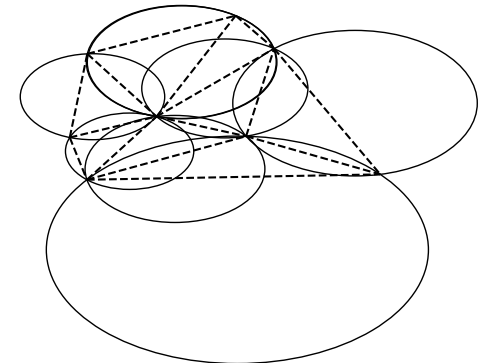
\includegraphics[width=0.7\textwidth]{circumcircle.png}
    \caption{Delaunay triangulations and their Circumcircles}
    \label{fig:my_label}
\end{figure}
\begin{theorem}[Optimality]
Over all proper $2D$ triangulations, the Delaunay triangulation maximizes the minimum angle of any triangle.
\end{theorem}
\begin{proof}
See \cite{FORTUNE1995} Theorem 3.1
\end{proof}
This implies that the Delaunay triangulation is the most equiangular one, which makes it computationally more desirable in finite element and interpolation methods \cite{Aurenhammer1991} \cite{Rebay1993}.
\subsection{Possible Algorithms}
Here follows a short overview on different types on algorithms. For convenience reasons we will present all algorithms in terms of the Delaunay triangulation instead of the Voronoi diagram, which is easily obtained from any graph-based Delaunay representation. For a more detailed discussion, see \cite{FORTUNE1995}.\\
The following bounds are known for computing Delaunay triangulations \cite{FORTUNE1995}:
\begin{itemize}
    \item For $2$ dimensional Delaunay triangulations, a worst case lower bound of $\Omega(n \log n)$ is known.
    \item For $d > 2$ dimensional Delaunay triangulations, an lower bound of $\Omega(n^{\lceil d/2 \rceil})$ is known.
\end{itemize}
\subsubsection{Flip Algorithm}
Flipping algorithms are the most simple type of algorithm. At first, you start with some kind of triangulation, which doesn't have any further constraints. From there on, we can just "flip" edges until every edge furfills the circumcircle property. The mapping from the starting triangulation to the ending one is called a \textbf{transformation}. Formally:
\begin{theorem}[flips and flippable edges]
Let $\Delta_1, \Delta_2$ be two neighbouring triangles with $e$ being the edge contained in both boundaries. If the union of both triangles $C := \Delta_1 \cup \Delta_2$ forms a convex quadrilateral, $e$ is \textbf{flippable}. \textbf{Flipping} $e$ means replacing $e$ with it's diagonal in $C$.
\end{theorem}
\begin{figure}[H]
    \centering
    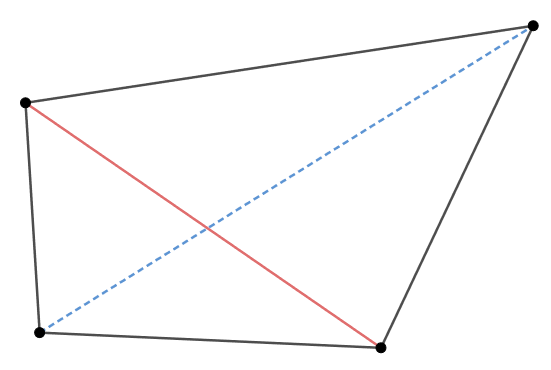
\includegraphics[width=0.7\textwidth]{flippable.png}
    \caption{A flippable edge (red), it's alternative (blue) and the required convex quadrilateral (black)}
    \label{fig:my_label}
\end{figure}
While this class of algorithms is conceptually very simple, it has very poor performance, with some transformations requiring at least $\Omega(n^2)$ flips \cite{Hurtado1999}.
\subsubsection{Incremental Algorithm}
The incremental algorithm works by using the circumcircle property inductively. It was first introduced for two dimensions by \cite{Green1978}, which was later generalized to $n$-dimensions by both \cite{Bowyer1981} and \cite{Watson1981} simultaneously.\\
We will inspect this algorithm in more rigorously in section 3.4, but the basic idea works as follows:
\begin{figure}[H]
    \centering
    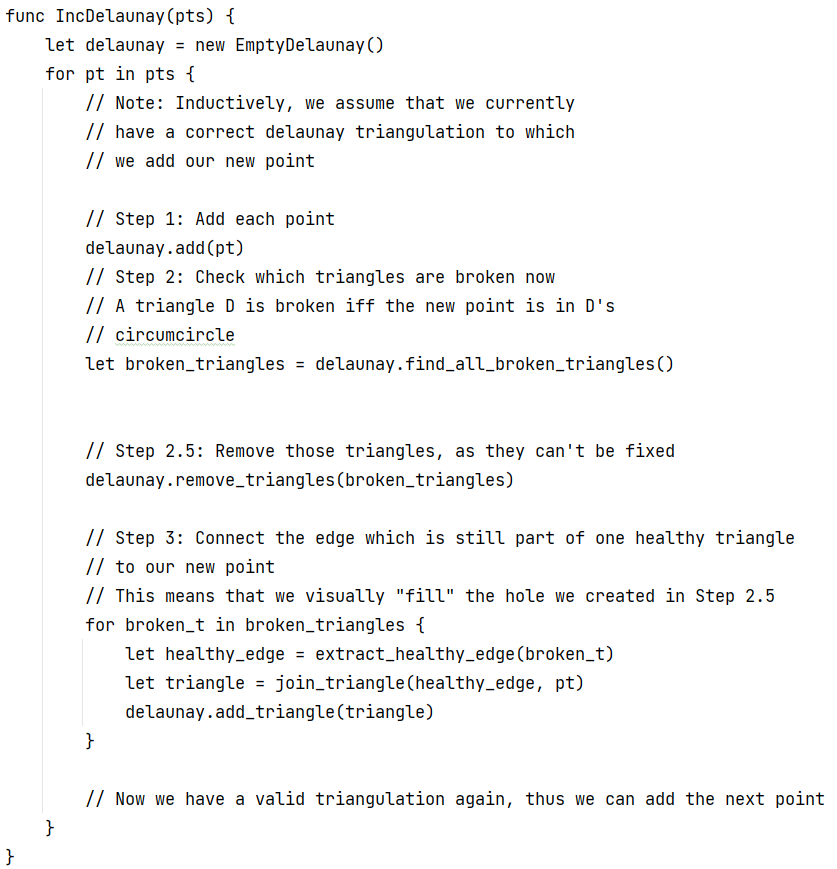
\includegraphics[width=\textwidth]{delaunayPseudocode.png}
    \caption{Pseudocode Green-Sibson/Bowyer/Watson}
    \label{fig:my_label}
\end{figure}
The average case time complexity is $O(n^{1 + 1/d})$ where $d$ is the number of dimensions \cite{Bowyer1981}.
% Runtime
\subsubsection{Divide and Conquer Algorithm}
A \textbf{Divide and Conquer} algorithm can be broken down into 3 steps:
\begin{enumerate}
    \item \textbf{Divide} the problem into smaller subproblems
    \item \textbf{Conquer} the subproblems by solving them recursively until they are small enough to be solvable straightforward.
    \item \textbf{Merge} the solutions of those smaller subproblems into the original problem
\end{enumerate}
This results in the following cost function
\[
T(n) := a\cdot T(n/b) + c(n)
\]
where
\begin{itemize}
    \item $a$ are the number of subproblems,
    \item $n/b$ is the size of the subproblem,
    \item $c(n)$ is the cost function matching the cost of the combine step.
\end{itemize}
This is equivalent to the following Pseudocode
\begin{figure}[H]
    \centering
    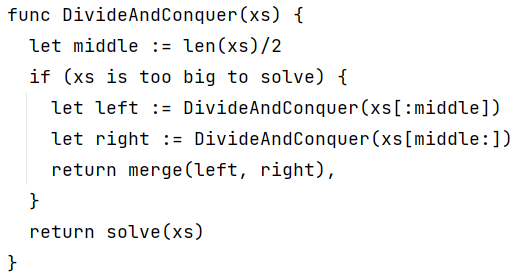
\includegraphics[width=0.7\textwidth]{pseudocode_dnc.PNG}
    \caption{Pseudocode D\&C}
    \label{fig:my_label}
\end{figure}
There are 2 ways to use the D\&C paradigm for constructing Delaunay Triangulations.
\newpage
The \textbf{naive way} would work as follows:
\begin{figure}[H]
    \centering
    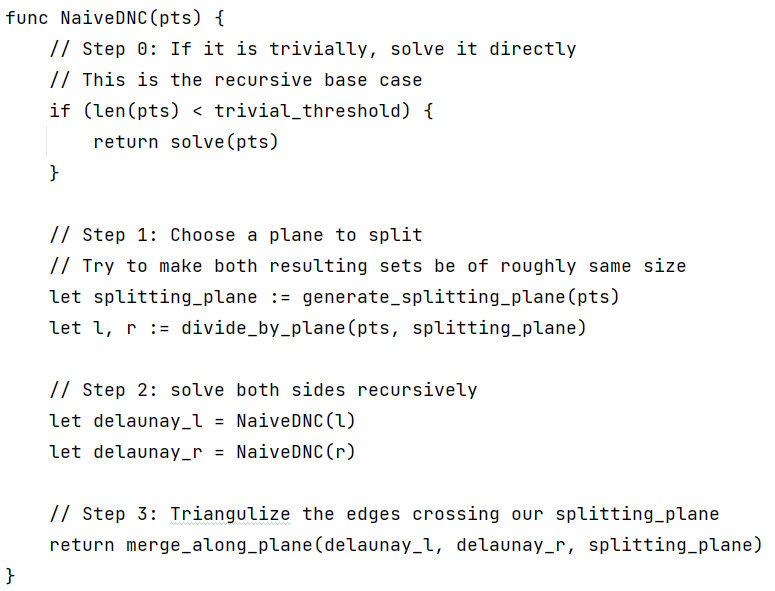
\includegraphics[width=\textwidth]{pseudocode_dnc_naive.PNG}
    \caption{Pseudocode D\&C for naively creating a Delaunay Triangulation}
    \label{fig:my_label}
\end{figure}
\begin{figure}[H]
     \centering
     \begin{subfigure}[b]{0.3\textwidth}
         \centering
         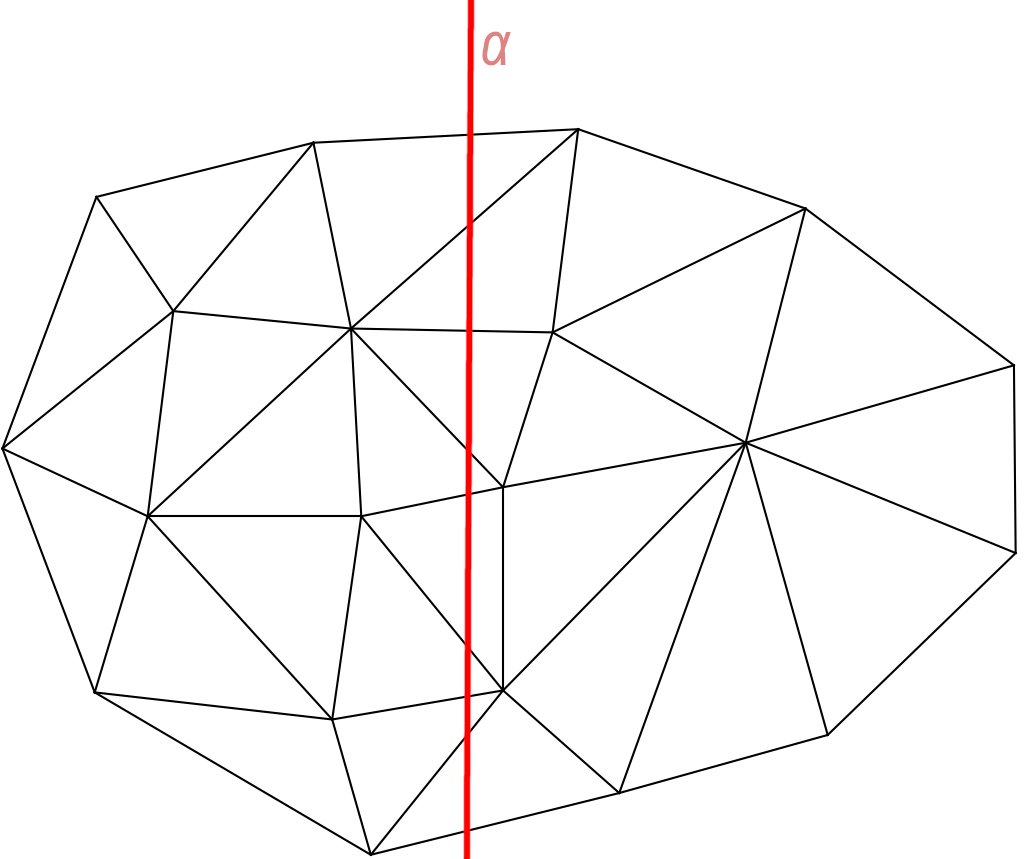
\includegraphics[width=\textwidth]{01NaiveCut.png}
         \caption{Divide into 2 subproblems}
         \label{fig:y equals x}
     \end{subfigure}
     \hfill
     \begin{subfigure}[b]{0.3\textwidth}
         \centering
         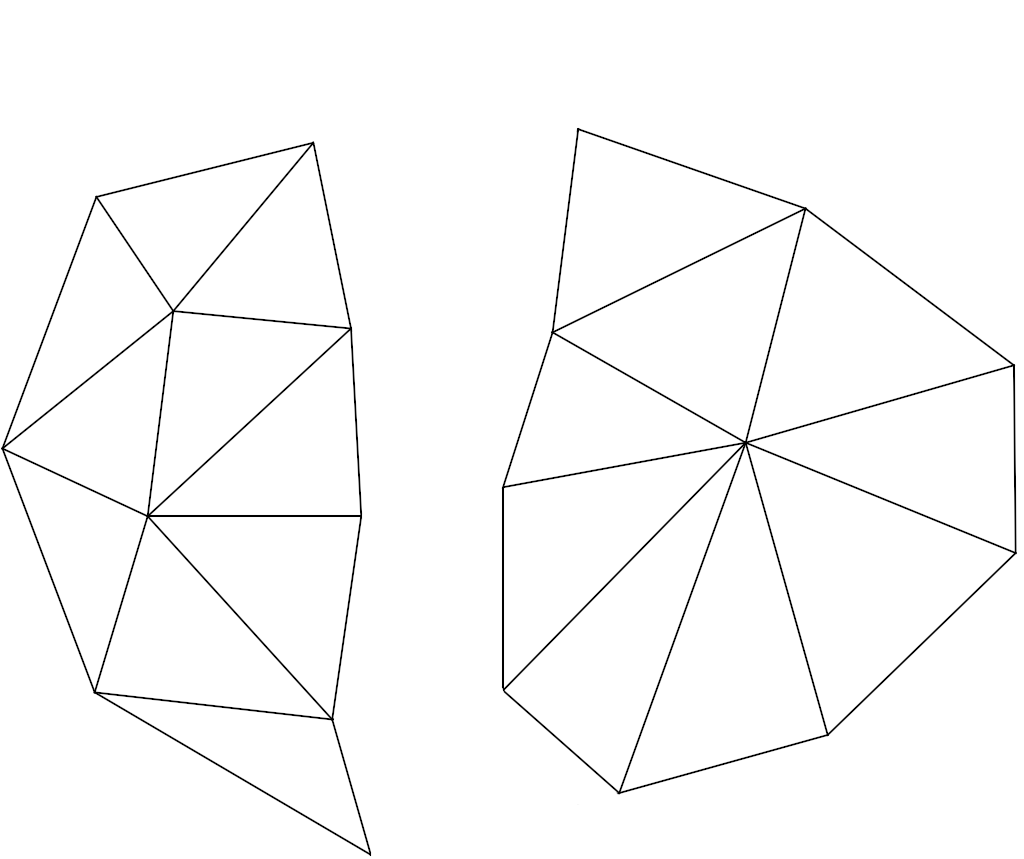
\includegraphics[width=\textwidth]{02NaiveSub.png}
         \caption{Solve the subproblems recursively}
         \label{fig:three sin x}
     \end{subfigure}
     \hfill
     \begin{subfigure}[b]{0.3\textwidth}
         \centering
         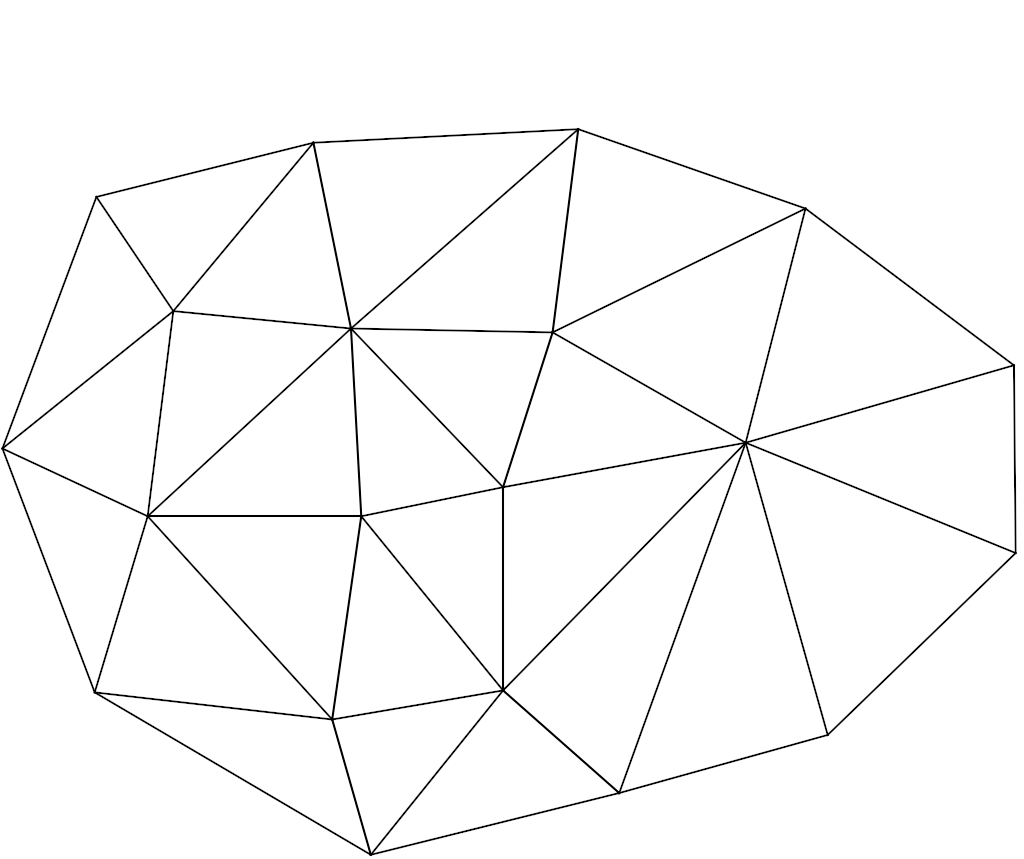
\includegraphics[width=\textwidth]{03SimpleConnectMiddle.png}
         \caption{Merge the subproblems}
         \label{fig:five over x}
     \end{subfigure}
        \caption{Naive D\&C Algorithm, Visually}
        \label{fig:three graphs}
\end{figure}
Note that, while merging both subproblems, this algorithm can still require additional changes to the already solved triangulations.\\
The better and more generalizable approach was first introduced by \cite{Cignoni1998}. The so-called \textbf{DeWall} algorithm can be simplified to the following idea:
\begin{figure}[H]
    \centering
    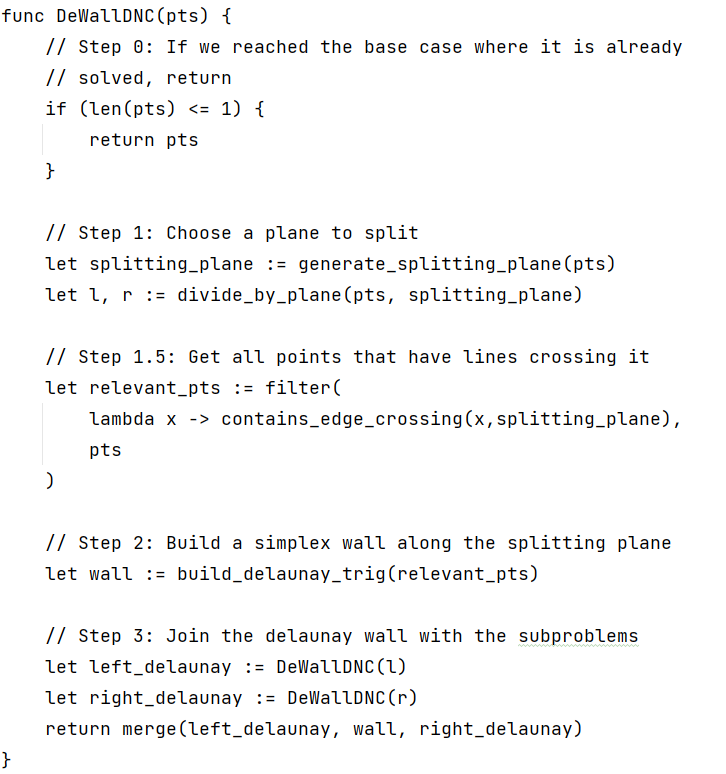
\includegraphics[width=\textwidth]{pseudocode_dnc_dewall.PNG}
    \caption{Pseudocode D\&C DeWall}
    \label{fig:my_label}
\end{figure}
\newpage
Visually:
\begin{figure}[H]
     \centering
     \begin{subfigure}[b]{0.3\textwidth}
         \centering
         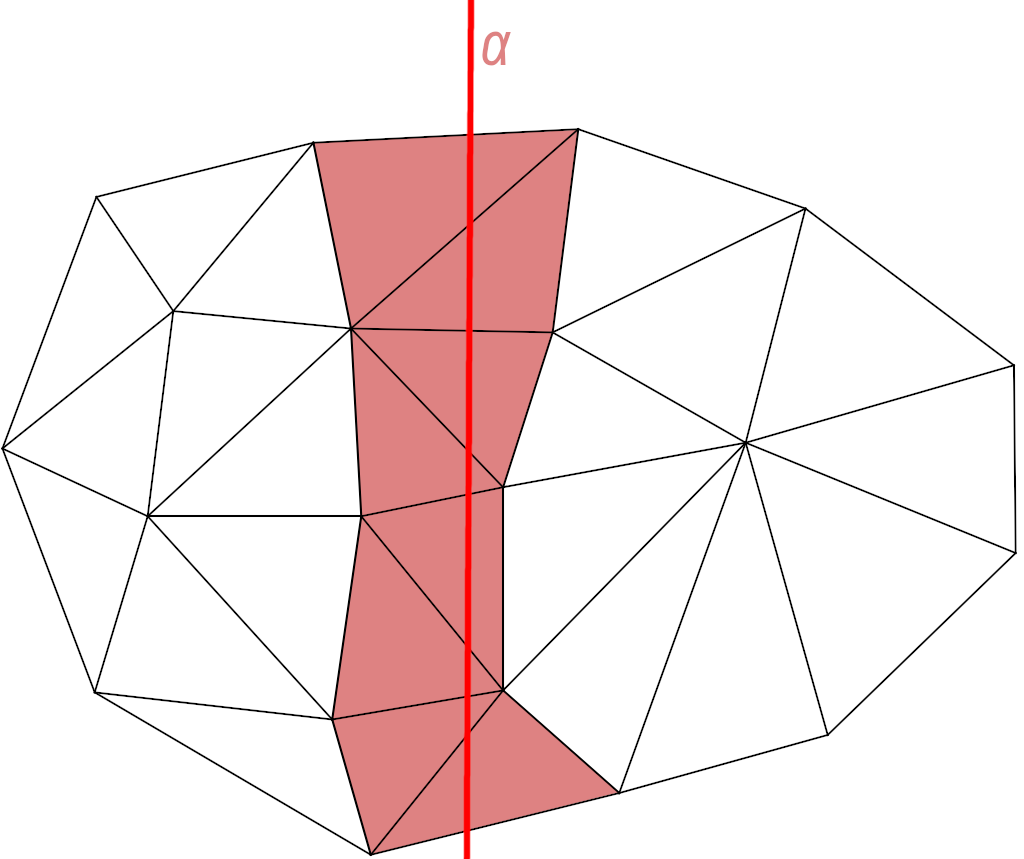
\includegraphics[width=\textwidth]{01DeWallMiddle.png}
         \caption{Cut into 2 problems}
         \label{fig:y equals x}
     \end{subfigure}
     \hfill
     \begin{subfigure}[b]{0.3\textwidth}
         \centering
         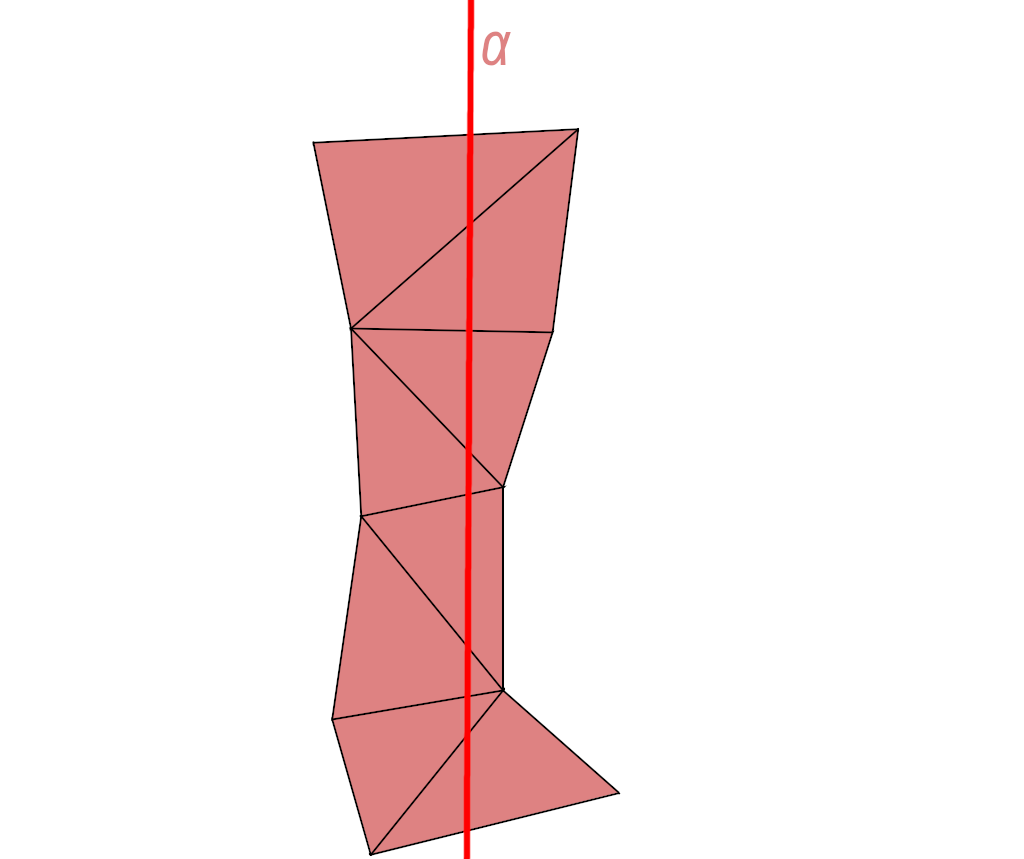
\includegraphics[width=\textwidth]{01DeWallSolveMiddle.png}
         \caption{Solve the Middle first}
         \label{fig:three sin x}
     \end{subfigure}
     \hfill
     \begin{subfigure}[b]{0.3\textwidth}
         \centering
         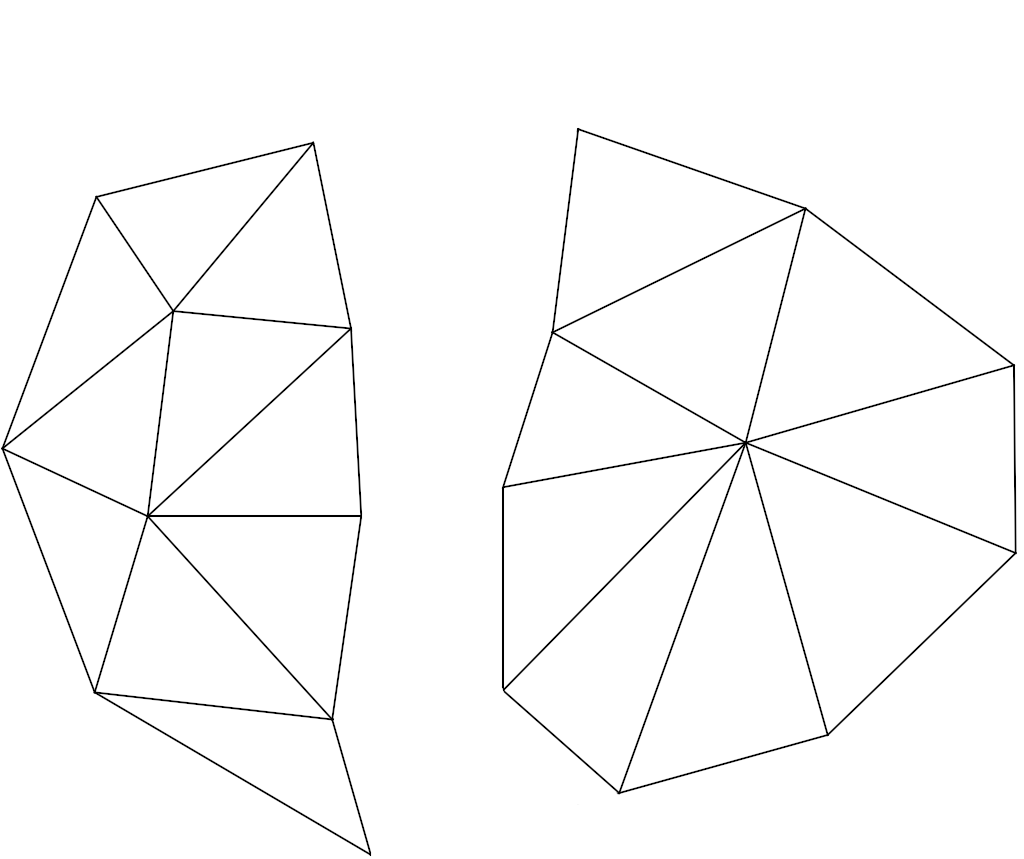
\includegraphics[width=\textwidth]{02NaiveSub.png}
         \caption{Solve the both sides recursively like (ii)}
         \label{fig:five over x}
     \end{subfigure}
        \caption{DeWall Algorithm, Visually}
        \label{fig:three graphs}
\end{figure}
The worst case time complexity of DeWall is known to be $O(n^{\lceil d/2 \rceil +1})$, with $d$ being the number of dimensions
\subsubsection{S-hull Algorithm}
The \textbf{S-hull} \cite{Sinclair2010} algorithm belongs to the family of the so-called line sweep algorithms, which describes solving a problem geometrically in an space by traversing it and working with distances. Note that this requires an euclidean norm.\\
\cite{Sinclair2010} contains a great pseudocode summary:
\begin{quote}
    S-hull operates as follows: For a set of unique points $x_i \in \mathbb{R}^2$:
    \begin{enumerate}
        \item select a seed point $x_i$ from $x_i$.
        \item sort according to $|x_i - x_0|^2$.
        \item find the point $x_j$ closest to $x_0$.
        \item find the point $x_k$ that creates the smallest circum-circle with $x_0$ and $x_j$ and record the center of the circumcircle $C$.
        \item order points $[x_0, x_j, x_k]$ to give a right handed system: this is the initial seed convex hull
        \item resort the remaining points according to $|x_i-C|^2$ to give points $s_i$.
        \item sequentially add the points $s_i$ to the porpagating 2D convex hull that is seeded with the triangle formed from $[x_0, x_j, x_k]$. As a new point is added the facets of the 2D-hull that are visible to it form new triangles.
        \item a non-overlapping triangulation of the set of points is created. (This is an extremly fast method for creating an non-overlapping triangulation of a 2D point set).
        \item adjacent pairs of triangles of this triangulation must be 'flipped' to create a Delaunay triangulation from the initial non-overlapping triangulation.
    \end{enumerate}
\end{quote}
This algorithm just works on 2D and it's worst case time complexity is $O(n\log n)$. 
\subsubsection{q-hull Algorithm}
\begin{definition}[Convex Set]
A Set $S$ is \textbf{convex} if, for all $x,y \in S$, the line segment $L_{x,y} := \{ tx+(1-t)y : t \in [0,1] \}$ is in $S$.
\end{definition}
\begin{definition}[Convex Hull]
A \textbf{Convex Hull} of a set of $N$ points is defined as the smallest convex set which contains all of the points.
\end{definition}
In $\mathbb{R}^2$, this is a convex polygon of at most $N$ sides.\\
\begin{theorem}[Delaunay Triangulation/Convex Hulls]
A Delaunay triangulation in $\mathbb{R}^d$ can be created by computing the convex hull in $R^{d+1}$, followed by then extracting the set of ridges of the lower convex hull.
\end{theorem}
\begin{proof}
Constructive proof, see \cite{Brown1979}.
\end{proof}
This is the most common way for computing Delaunay triangulation, as most numerical libraries like Scipy \cite{Scipy2022} use the qhull library \cite{QHull} based on the Quickhull Algorithm \cite{Barber1996}.
\subsection{Our Algorithm and Implementation}
We chose to implement an incremental algorithm which is a simplified version of \cite{Green1978}, which in itself is a $2$ dimensional version of \cite{Bowyer1981} and \cite{Watson1981}, in which finding the triangle containing a new point takes $O(n)$, instead of the $O(\sqrt{n})$ neighbour walk alleged by \cite{Bowyer1981}.
\subsubsection{Basic Idea}
As mentioned before, all incremental algorithms work inductively by assuming a valid Delaunay triangulation of $n-1$ points, adding the $n$-th point, then repairing the triangulation afterwards.
\newpage
\cite{Rebay1993} summarizes the algorithm as follows:
\begin{quote}
    The method is based on the so-called \textit{circumcircle property} which guarantees that no point of a Delaunay triangulation can lie within the circle circumscribed to any triangle. The Bowyer-Watson algorithm is essentially a "reconnection" method, since it computes how an existing Delaunay triangulation is to be modified because of a new point.
\end{quote}
\subsubsection{A visual example}
Assume we have generated the following valid Delaunay triangulation of $n-1$ points:
\begin{figure}[H]
    \centering
    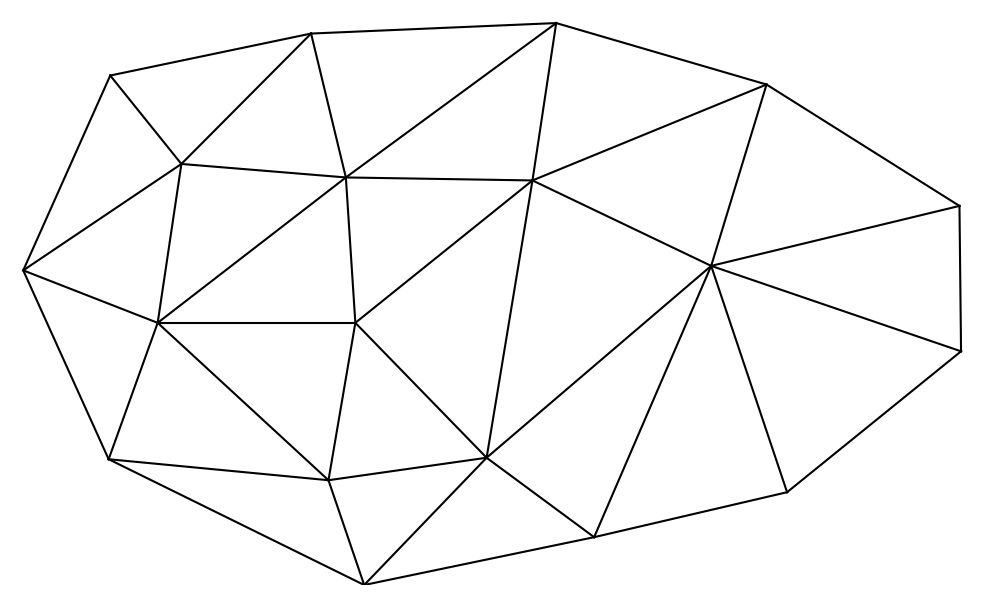
\includegraphics[width=0.6\textwidth]{DelaunayVisualExample01.png}
\end{figure}
Now we want to add a new point into this triangulation.
\begin{figure}[H]
    \centering
    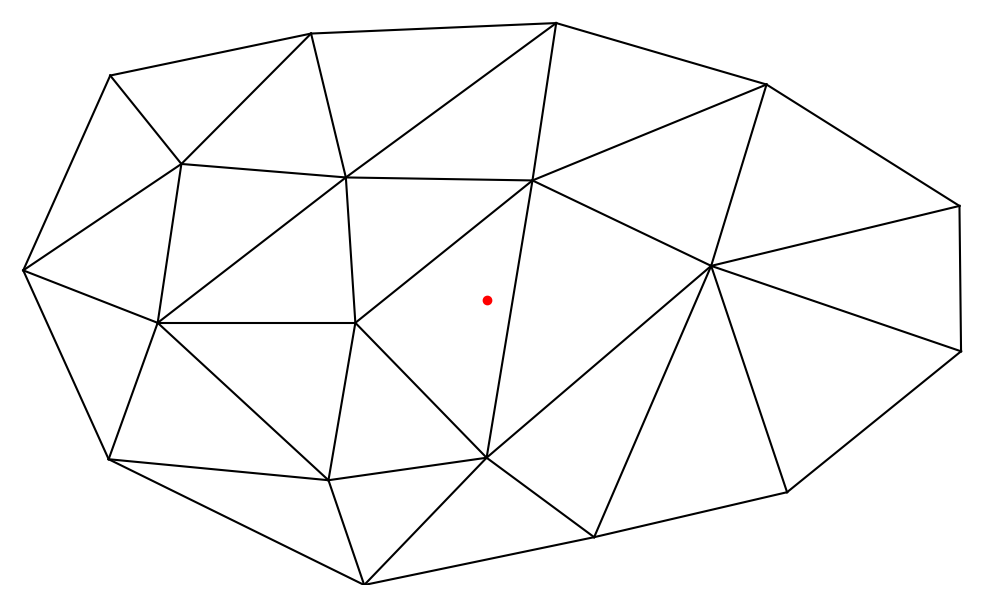
\includegraphics[width=0.6\textwidth]{DelaunayVisualExample02.png}
\end{figure}
The circumcircle property shows us that any valid Delaunay triangulation has no other points in the circumcircles spanned by all triangles. This also means that any triangle that contains our new point can't be valid!\\
Note that we just have to focus on our newly inserted point since we know that we started with an already valid Delaunay triangulation.
\newpage
Let's look at the circumcircles:
\begin{figure}[H]
    \centering
    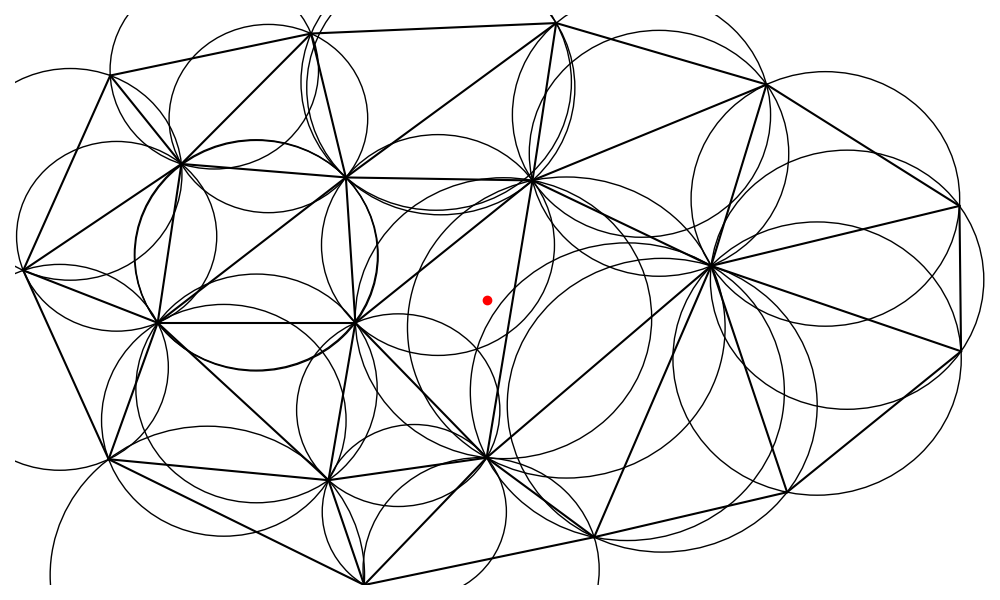
\includegraphics[width=0.6\textwidth]{DelaunayVisualExample03.png}
\end{figure}
Now just show the invalid ones:
\begin{figure}[H]
    \centering
    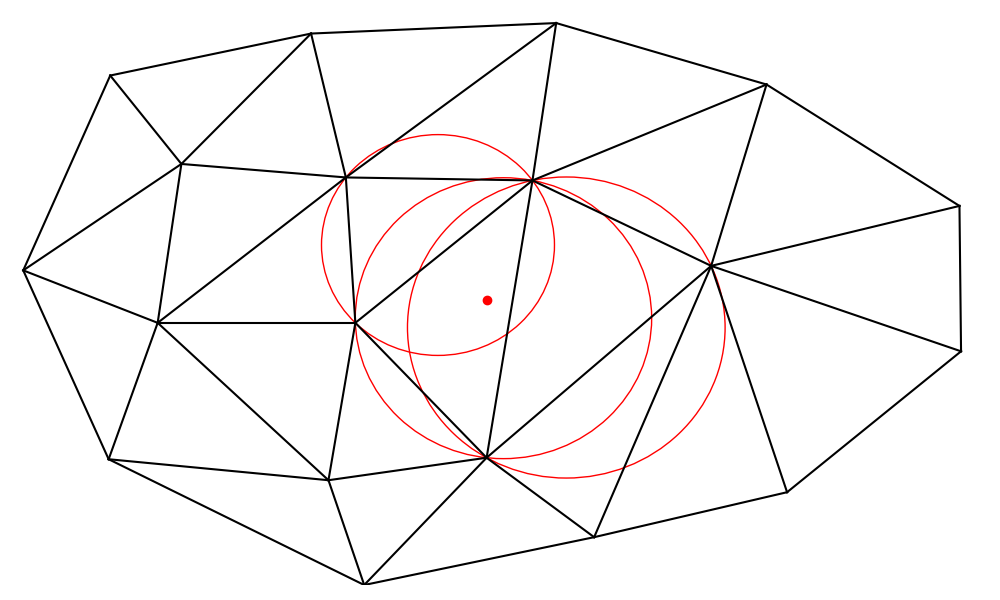
\includegraphics[width=0.6\textwidth]{DelaunayVisualExample04.png}
\end{figure}
We now know that those triangles are broken. Thus we remove them.
\begin{figure}[H]
    \centering
    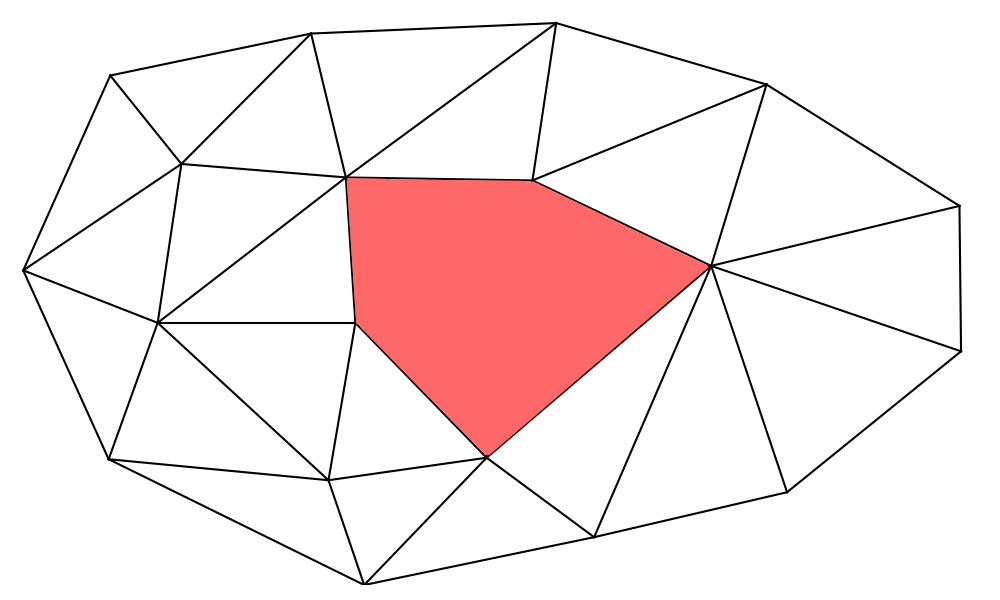
\includegraphics[width=0.6\textwidth]{DelaunayVisualExample05.png}
\end{figure}
Now we only have one valid way to fill the hole: Connecting all leftover edges to our new point. This makes sense intuitively, since this way results in the most equilateral triangles, thus furfilling Delaunay's optimality criteria. Formally, we know that a triangulation is Delaunay if and only if it is locally Delaunay, which means that any non-optimal solution wouldn't be possible (\cite{FORTUNE1995}, Lemma 2.2).\\
So let us reconnect them:
\begin{figure}[H]
    \centering
    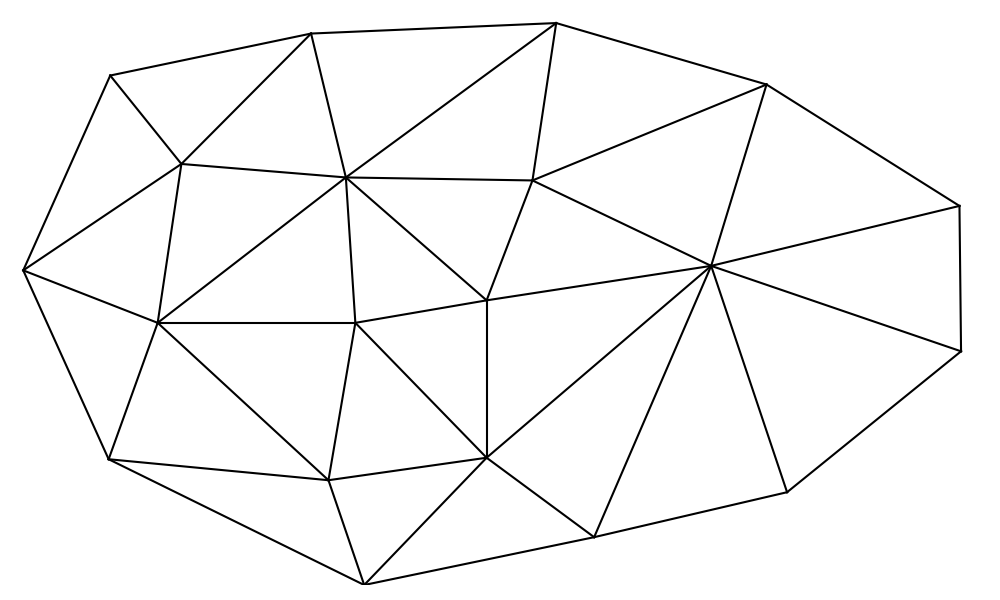
\includegraphics[width=0.6\textwidth]{DelaunayVisualExample06.png}
\end{figure}
Now we have a valid triangulation of $n$ points. To verify, here are all circumcircles:
\begin{figure}[H]
    \centering
    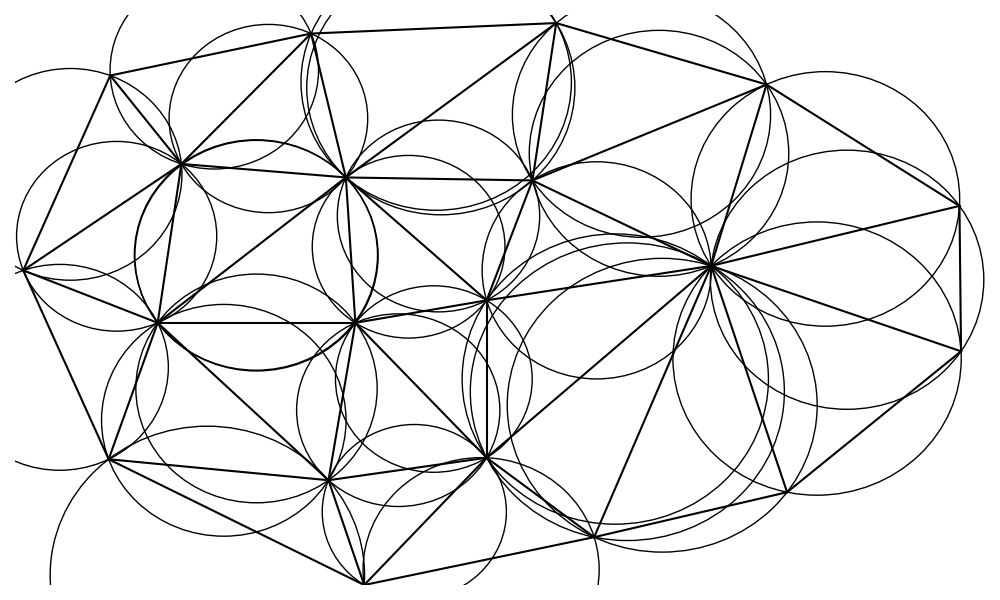
\includegraphics[width=0.6\textwidth]{DelaunayVisualExample07.png}
\end{figure}
And for clarity, just the new circumcircles:
\begin{figure}[H]
    \centering
    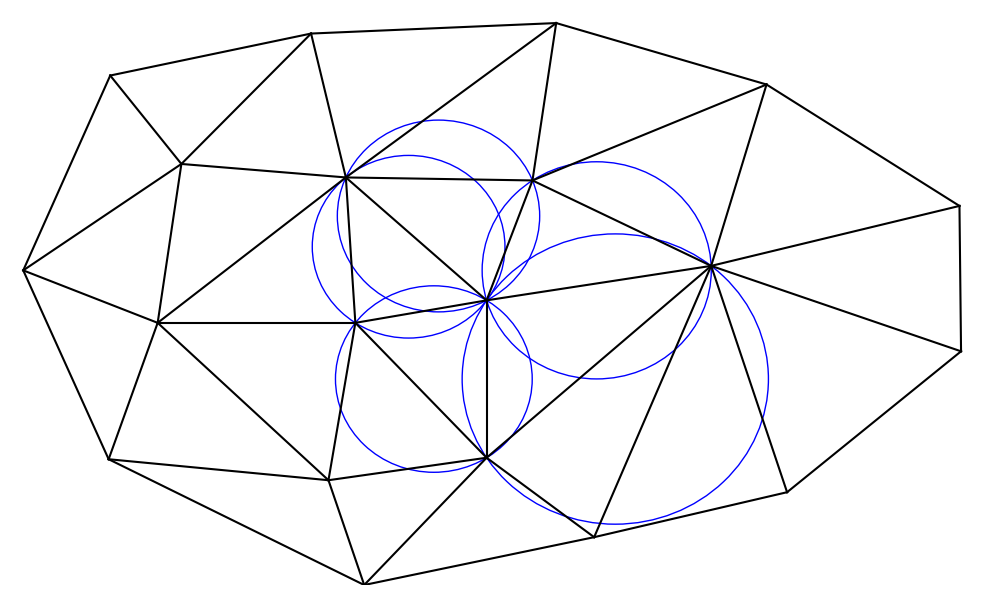
\includegraphics[width=0.6\textwidth]{DelaunayVisualExample08.png}
\end{figure}
Now all are valid again, resulting in a new Delaunay triangulation
of $n$ points.
\subsubsection{Initial State}
The incremental method works inductively and as we have just seen our induction step is correct. Now we have to handle the base case. This is more difficult because any set with less than 3 points is not triangularizable.\\
In order to make it easier, we use Green-Sibson's window \cite{Green1978} and extend it with a supertriangle \cite{PyDelaunay}.
\begin{definition}[Window]
A \textbf{window} is a axially parallel rectangle which contains all points of the Delaunay triangulation.
\end{definition}
Now we also have to extend our Voronoi tile definition:
\begin{definition}[Window-aware Voronoi tiles]
Let $\mathcal{P}_N := \{P_1,\dots, P_N\}$ be finitely many points in the plane such that $P_i \neq P_j, i \neq j$.  Further let $E$ be a window such that all points fit. The \textbf{window-aware Voronoi tile} of $P_i$ is the set $T_i^*$ defined by
\[
T_n^* := \{ x \in E : d(x, P_i) < d(x, P_j) \forall i \neq j, P_j \in E  \}
\]
In our algorithm, all Voronoi tiles are window-aware.
\end{definition}
The window used in our algorithm is square. This window allows us to have a boundary, in which all points are contained. In order to make the window a valid triangulation we extend it to a super-triangle:
\begin{definition}[Supertriangle]
A \textbf{supertriangle} is a window with an additional diagonal edge, dividing it into 2 triangles.
\end{definition}
\begin{figure}[H]
    \centering
    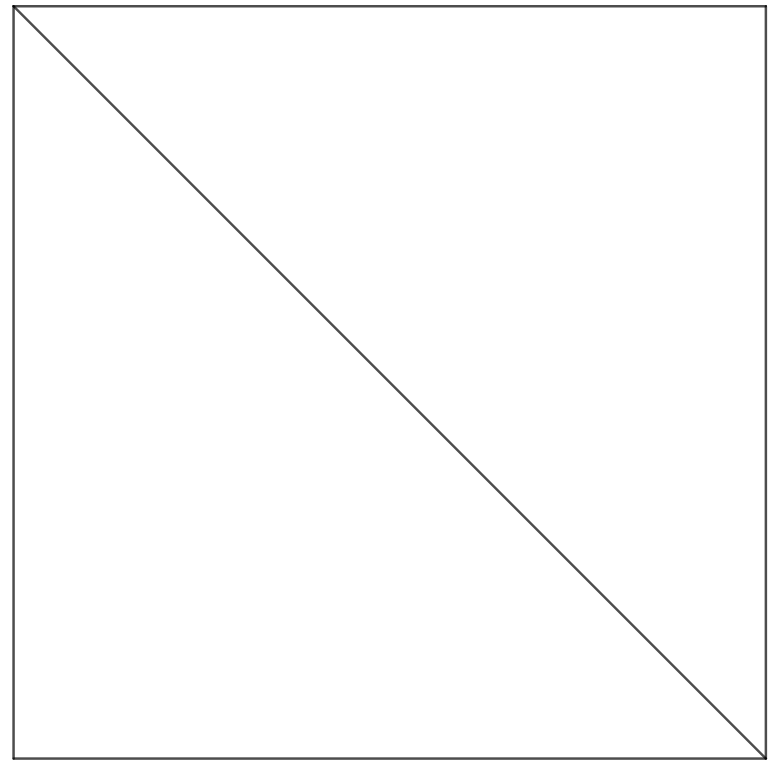
\includegraphics[width=0.5\textwidth]{supertriangle.png}
    \caption{Supertriangle, all points outside of it are invalid}
    \label{fig:my_label}
\end{figure}
This supertriangle is only used internally; all edges and vertices are not part of the Delaunay triangulation.
\subsubsection{Mesh Data Structure}
The most important part of this algorithm is fast graph traversal, thus we heavily rely on a efficient mesh data structure. Our data structures are defined as follows:
\begin{figure}[H]
    \centering
    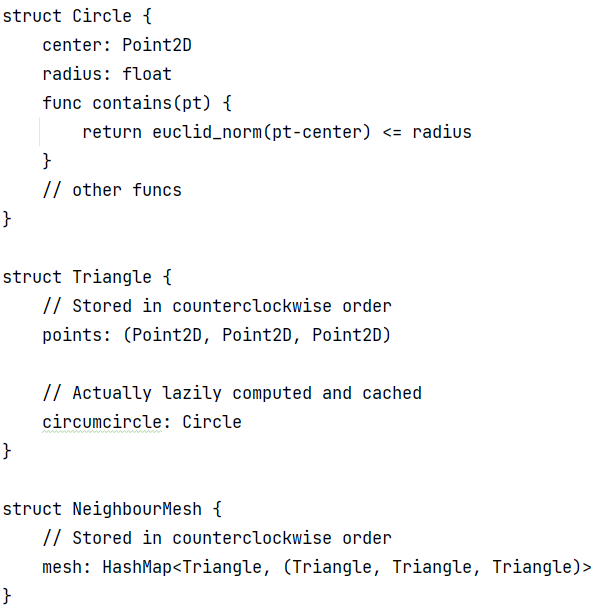
\includegraphics[width=\textwidth]{ds.png}
\end{figure}
The Mesh gets updated while adding new points.\\
This Data structure has multiple great properties:
\begin{itemize}
    \item Since we only have 2 dimensions and have the circle as a member variable, detecting whether a point lies in a triangles circumcircle is $\Theta(1)$.
    \item Although Python dictionaries (i.e. Hashmaps) use open hashing, our hash function is chosen in a way that the hash seed of two triangles is only equal if and only if they share all 3 points. Thus our triangle lookup results in $\Theta(1)$.
    \item Since any triangle only has 3 neighbours, we can traverse $n$ triangles in $\Theta(n)$, which is obviously optimal.
\end{itemize}
\subsubsection{Triangle Replacement Optimization}
In order to optimize the triangle replacement we use 2 useful properties from \cite{Rebay1993}:
\begin{quote}
    The algorithm removes from the existing grid all the triangles which violate the circumcircle property because of the insertion of the new point.\\
    It can be shown that
    \begin{enumerate}
        \item all these triangles are always contiguous, thus forming a connected cavity surrounding the newly inserted point, and that
        \item by joining the vertices of the cavity with the internal new point, a Delaunay triangulation is always obtained.
    \end{enumerate}
\end{quote}
Our optimization thus consists of three parts:
\begin{itemize}
    \item The aforementioned $O(1)$ traversal neighbour mesh data structure
    \item Remembering which edges need to be reconnected while deleting the broken triangles
    \item Only traversing along the hole edges, starting at a random edge. This works because we know that the hole is contiguous.
\end{itemize}
\newpage
\subsubsection{Triangle Replacement Implementation}
This is the code for adding a new point to the Delaunay triangulation:
\begin{figure}[H]
    \centering
    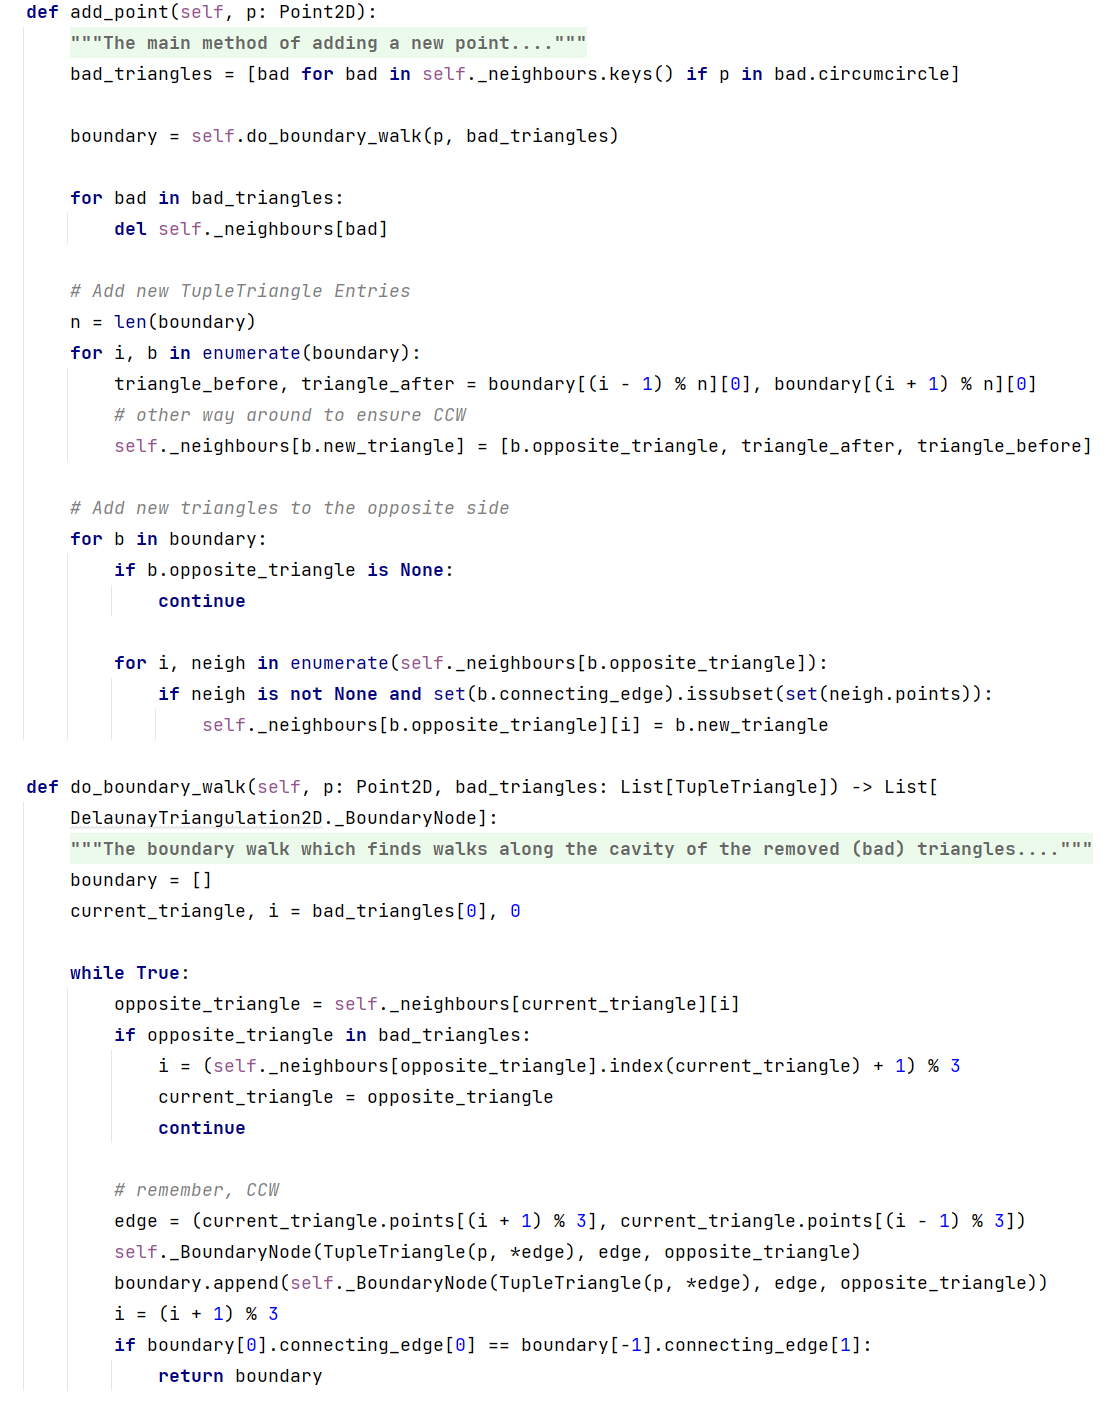
\includegraphics[width=\textwidth]{add_point_full.png}
\end{figure}
It works as follows:
\begin{itemize}
    \item At first, we detect all broken triangles by checking their circumcircles
    \item Now we do the \textbf{boundary walk} that works as follows:\\
    We start at any triangle. Note that we cannot yet know whether it is entirely surrounded by broken triangles or not. We choose any edge of it.\\
    Then we rotate along the edges counter clock wise (CCW) and go to the triangle that is connected to our triangle through this edge. One can see that through this motion we go in a more or less specific direction.\\
    Eventually (in reality it's pretty fast, \cite{Green1978} shows that through the Euler-Poincare formula) we reach an edge that is connected to a valid triangle (i.e. a triangle which circumcircle contains only it's 3 points). This is relevant because we have to reconnect the edge connecting the broken and valid triangle to our new point.\\
    We call this edge-path of valid-to-invalid triangles our \textbf{boundary}.\\
    Now, by moving counter clock wise, we stay along the boundary. We record not only every boundary edge, but also to which boundary edges it is connected to. This allows for linear time insertion of the new triangles since we do not have to search the neighbour (which, combinatorically, would result in $O(n^2)$ where $n$ is the number of boundary edges).
    \begin{figure}[H]
    \centering
    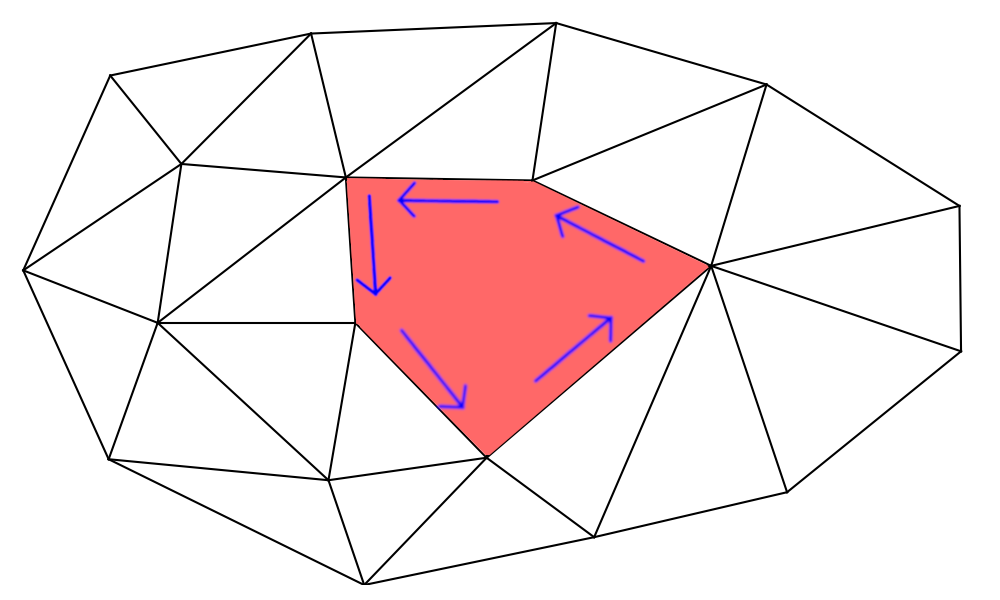
\includegraphics[width=0.5\textwidth]{ccwBoundaryWalk.png}
    \caption{CCW walk. We always check that we are connected to one valid and one broken triangle}
    \label{fig:my_label}
    \end{figure}
    Note: the neighbours do not have to be saved explicitly. Since it is a list, and we add it one by one while walking along the neighbourship, it is implicitly ordered.\\
    We stop once we meet our first boundary triangle again (we ran a circle).\\
    \textit{This is the main algorithm optimization}.
    \item After collecting the boundary, we can delete all broken triangles.
    \item Lastly, we walk along the boundary and create new triangles, consisting the boundary edge connected to our new point. Note that we can add the triangle neighbours in $O(1)$ because our boundary is ordered (see the traversal).
\end{itemize}
\subsection{Runtime Analysis}
The initial data structure creation is $\Theta(1)$. For each point, we have the following costs for adding the $n$-th point:
\begin{enumerate}
    \item To detect all broken triangles, we look at all triangles. As explained in the data structure section, this lookup is $\Theta(1)$, resulting in $\Theta(n)$
    \item The boundary walk takes $\Theta(1)$ per triangle. Thus we can choose an upper bound of $O(n)$, although this bound is not very tight.
    \item Deleting a bad triangle takes $\Theta(1)$. Thus $\Theta(1) \cdot |\text{\texttt{bad\_triangles}}| \in O(n)$.
    \item Connecting one boundary edge with the new point, creating a new triangle and updating our neighbour mesh all takes $\Theta(1)$. Again, its upper bound is $O(n)$
\end{enumerate}
Resulting in a runtime of $\Theta(n) + 3 \cdot O(n) = O(n)$ per point.\\
If we have $m$ points, this results in $O(m^2)$.
\subsubsection{Possible Improvements and Beyond}
As shown by Bowyer-Watson \cite{Bowyer1981} \cite{Watson1981}, this algorithm could theoretically be generalized to $n$ dimensions.\\
Both Green-Sibson \cite{Green1978}, Bowyer \cite{Bowyer1981} and \cite{Rebay1993} alledge that the nearest-neighbour search (i.e. finding the triangle our new point is contained in) can be implemented in $O(n^{1/d})$ with $d$ being the dimension. Sadly, this was never proven rigorously \cite{FORTUNE1995}. Also, no algorithm is mentioned in the literature. For now, the question on whether this is actually possible remains open \cite{CSSE}.